\chapter{Regler- und Systemmatrizen}\label{app:matrizen}
Die Systemmatrizen für das nominelle System lauten
\begin{equation*}
\textbf{A} = \begin{bmatrix} 
-0.0426 & 0 & -0.008282 & 0 & 10.81 & 0 & 0 & -9.784 & 0.0003409\\ 
0 & -0.208 & 0 & -11.02 & 0 & -150.0 & 9.784 & 0 & 0\\
-0.1844 & 0 & -0.7339 & 0 & 147.1 & 0 & 0 & 0.7189 & 0.001059\\
0 & -0.09575 & 0 & -4.888 & 0 & 2.321 & 0 & 0 & 0\\
-0.002906 & 0 & -0.02645 & 0 & -1.143 & 0 & 0 & 0 & 7.811e-6\\
0 & 0.03642 & 0 & 0.4039 & 0 & -2.089 & 0 & 0 & 0\\
0 & 0 & 0 & 1.0 & 0 & -0.07348 & 0 & 0 & 0\\ 
0 & 0 & 0 & 0 & 1.0 & 0 & 0 & 0 & 0\\ 
-0.07329 & 0 & -0.9973 & 0 & 0 & 0 & 0 & 150.4 & 0 \\
\end{bmatrix}
\end{equation*}

\begin{equation*}
\textbf{B} = \begin{bmatrix}
-1.009 & 9.81 & 0 & 0\\ 0 & 0 & 0 & 4.329\\ -13.73 & 0 & 0 & 0\\ 0 & 0 & -6.056 & 2.354\\ -5.333 & 0.2912 & 0 & 0\\ 0 & 0 & 0.1267 & -2.596\\ 0 & 0 & 0 & 0\\ 0 & 0 & 0 & 0\\ 0 & 0 & 0 & 0 \\
\end{bmatrix}.
\end{equation*}
Numerisch sehr kleine Werte $<10^{-09}$ werden aus Gründen der numerischen Stabilität nicht aus den Systemmatrizen entfernt. Für die Reglermatrizen gilt das Gegenteil. Da wie bereits zuvor erwähnt das Entfernen von sehr kleinen Werten $<10^{-09}$ aus den Reglermatrizen unerwarteter Weise zu numerischen Berechnungsproblemen und damit zu Optimierungsabbrüchen führt, werden diese nicht entfernt.
\begin{equation*}
\mat{F}_\tn{mod} = 
\begin{bmatrix}
1.8102\eexp{-13} & 1.5337\eexp{-13} & -171.2109 & 4.4174\eexp{-04}; \\
3.0748\eexp{-12} & 3.4751\eexp{-12} & -3111.7757 & 0.0320; \\
0.1382 & -0.9011 & 4.7167\eexp{-12} & -1.3999\eexp{-14}; \\
0.3295 & -1.3869\eexp{-13} & -8.5272\eexp{-12} & -8.3947\eexp{-14}; \\
-5.5453\eexp{-13} & 2.3767\eexp{-13} & -166.1567 & 3.8831\eexp{-04}; \\
-1.0261\eexp{-11} & 5.1066\eexp{-12} & -3015.8835 & 0.0310; \\
0.1383 & -0.9021 & 5.8368\eexp{-12} & -1.3996\eexp{-14}; \\
0.3299 & -1.3906\eexp{-13} & -8.6262\eexp{-12} & -8.4039\eexp{-14}
\end{bmatrix}
\end{equation*}

\begin{equation*}
\mat{K}_\tn{koppel} = 
\begin{bmatrix}
0.2181 & 1.3670\eexp{-07} & -0.0101 & -6.6039\eexp{-09} & ... \\
-0.6069 & 4.8960\eexp{-10} & 3.5613\eexp{-08} & -1.3294 & ... \\
-0.0013 & 1.1667\eexp{-05} & -1.3670\eexp{-07} & 1.5900\eexp{-04} & ... \\
6.6050\eexp{-09} & 2.7366\eexp{-04} & -4.8759\eexp{-10} & -3.5613\eexp{-08} & ... \\
5.5512\eexp{-04} & 5.2847\eexp{-05}; & & \\ 
3.9833 & -7.5467\eexp{-09} & -0.2863 & 3.8470\eexp{-10} & ... \\ 
0.0357 & 5.0982\eexp{-11} & -1.9650\eexp{-09} & 0.1041 & ... \\
-7.4242\eexp{-04} & 4.0686\eexp{-04} & 7.5498\eexp{-09} & 0.0055 & ... \\
-3.6007\eexp{-10} & 2.8206\eexp{-04} & -2.4985\eexp{-11} & 1.9668\eexp{-09} & ... \\
0.0066 & 2.3179\eexp{-04}; & & \\ 
1.06151\eexp{-09} & 0.1294 & 1.444\eexp{-08} & -1.7276 & ... \\
1.0361\eexp{-10} & -14.8366 & -0.0207 & -7.6591\eexp{-11} & ... \\
1.0636\eexp{-07} & -1.0599\eexp{-09} & 0.0048 & -1.4445\eexp{-08} & ... \\
0.0616 & -1.0366\eexp{-10} & -0.0045 & 0.0677 & ... \\
5.9533\eexp{-11} & -1.0636\eexp{-07}; & & \\
-7.6565\eexp{-10} & 0.4811 & -1.0419\eexp{-08} & -2.4372 & ... \\
3.1464\eexp{-11} & -34.6613 & 1.3199 & -3.5873\eexp{-11} & ... \\
-3.6855\eexp{-08} & 7.6455\eexp{-10} & -0.1995 & 1.0419\eexp{-08} & ... \\
-0.1092 & -3.1506\eexp{-11} & 0.0080 & 0.94028 & ... \\
4.7949\eexp{-11} & 3.6855\eexp{-08}; & & \\
-3.0300\eexp{-05} & -1.3665\eexp{-07} & -4.1234\eexp{-04} & 6.5917\eexp{-09} & ... \\
-3.3363\eexp{-04} & -4.8802\eexp{-10} & -3.5574\eexp{-08} & -5.76058\eexp{-04} & ... \\
5.3260\eexp{-05} & 0.2115 & 1.3665\eexp{-07} & -0.0102 & ... \\
-6.5912\eexp{-09} & -0.6073 & 4.8487\eexp{-10} & 3.5574\eexp{-08} & ... \\
-1.3312 & -0.0013; & & \\ 
-4.0613\eexp{-04} & 7.5514\eexp{-09} & -0.0055 & -3.6580\eexp{-10} & ... \\
-2.8814\eexp{-04} & -3.6877\eexp{-11} & 1.9671\eexp{-09} & -0.0068 & ... \\
2.5437\eexp{-04} & 3.8598 & -7.5616\eexp{-09} & -0.2879 & ... \\
3.7587\eexp{-10} & 0.0352 & -3.9288\eexp{-12} & -1.9660\eexp{-09} & ... \\
0.0907 & -7.5648\eexp{-04}; & & \\ 
-1.0601\eexp{-09} & 0.0048 & -1.4426\eexp{-08} & 0.0611 & ... \\
-1.0270\eexp{-10} & -0.0044 & 0.0676 & 7.6570\eexp{-11} & ... \\
-1.0624\eexp{-07} & 1.0585\eexp{-09} & 0.1295 & 1.4426\eexp{-08} & ... \\
-1.7282 & 1.0265\eexp{-10} & -14.8511 & -0.0207 & ... \\
-5.9604\eexp{-11} & 1.0624\eexp{-07}; & & \\ 
7.6471\eexp{-10} & -0.1990 & 1.0406\eexp{-08} & -0.1090 & ... \\
-3.1093\eexp{-11} & 0.0080 & 0.9415 & 3.5545\eexp{-11} & ... \\
3.6809\eexp{-08} & -7.6361\eexp{-10} & 0.4809 & -1.0407\eexp{-08} & ... \\
-2.4364 & 3.1097\eexp{-11} & -34.6993 & 1.3211 & ... \\\\
-4.7764\eexp{-11} & -3.6809\eexp{-08} & &
\end{bmatrix}
\end{equation*}

\chapter{Visualisierung}\label{app:Visual}
Der nachfolgende Abschnitt beschäftigt sich mit Möglichkeiten der Flugvisualisierung. Hierfür werden verschiedene in \MatSim implementierbare Methoden vorgestellt, mit deren Hilfe die Bewegungen von Flugzeugen dargestellt werden kann. 
Außerdem sollen Probleme beschrieben werden, welche im Zusammenhang mit dieser Arbeit aufgetreten sind. 
\section{Matlab interne Visualisierung}\label{app:VisualMat}
Zunächsten sollen die \MatSim internen Methoden dargestellt werden.
Die Basis bildet dabei die Aerospace Toolbox von \MatSim

In Abbildung \ref{fig:Sim6DoFBlock} ist vorgefertigter Block \cite{Sim6DoFDoku}. Dieser erstellt anhand der Eulerwinkel sowie den Koordinaten $\wt{X}{e} = \begin{bmatrix}x_e &y_e &z_e \end{bmatrix}^{\textnormal{T}}$ im erdfesten Koordinatensystem eine Animation der Flugzeugbewegung.
Wie in \ref{fig:Sim6DoFBlockMenuBsp} erkennbar kann über die Blockparameter die Anzahl an Flugobjekten und deren Geometrie definiert werden. Zudem kann man den Blickwinkel und die relative Position der Kamera vorgeben. 
%\begin{figure}[h]
%	\centering
%	\begin{subfigure}[b]{0.15\textwidth}
%		\centering
%		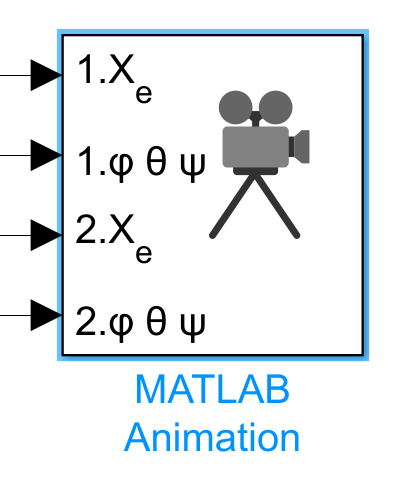
\includegraphics[width=\textwidth]{./Bilder/Visual_SimBlock.png}
%		\caption{Vorgefertigter 6DoF-Animations-Block}
%		\label{fig:Sim6DoFBlock}
%	\end{subfigure}
%	\hspace{0.1\textwidth}
%	\begin{subfigure}[b]{0.35\textwidth}
%		\centering
%		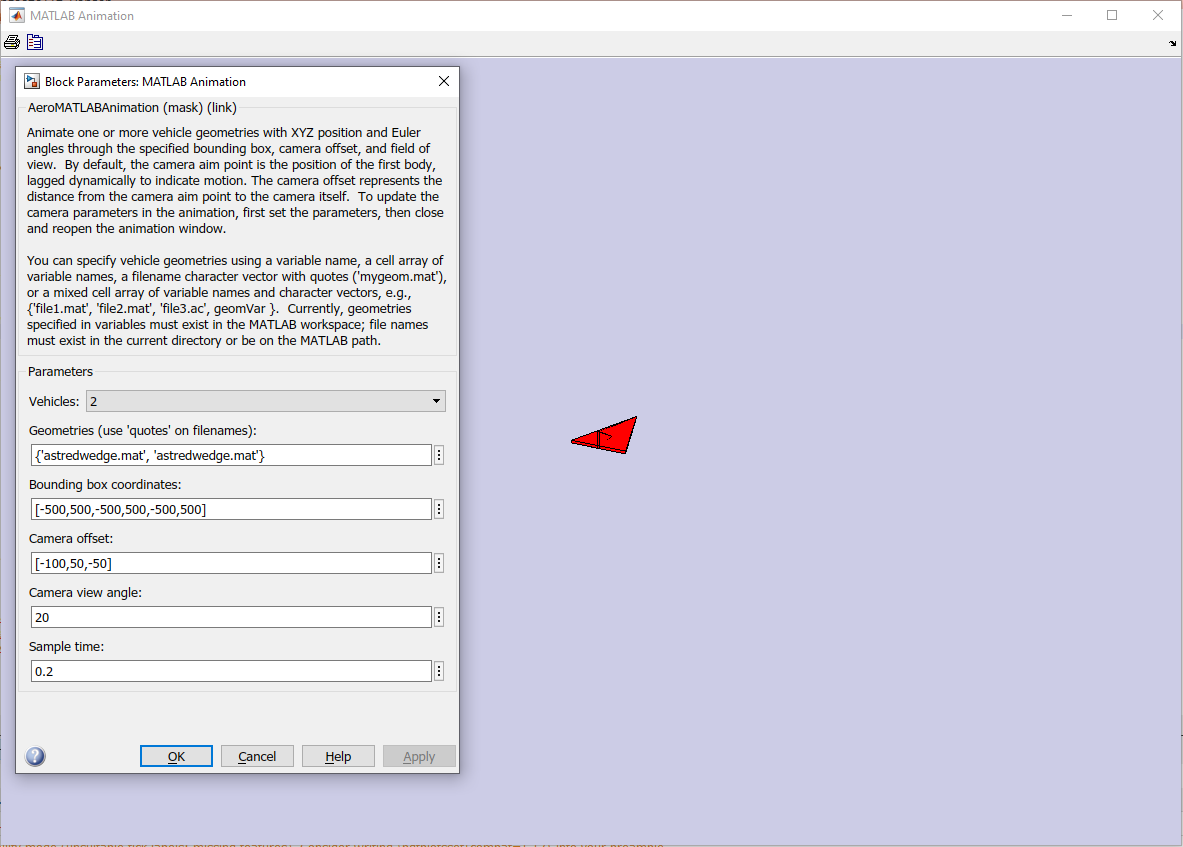
\includegraphics[width=\textwidth]{./Bilder/Visual_Sim6DoFBlockMenuBsp.png}
%		\caption{Blockparameter und Beispielanimation}
%		\label{fig:Sim6DoFBlockMenuBsp}
%	\end{subfigure}
%	\caption{Sim6DoFBlock}
%	\label{fig:Sim6DoF}
%\end{figure}
\begin{figure}[H]
	\centering
	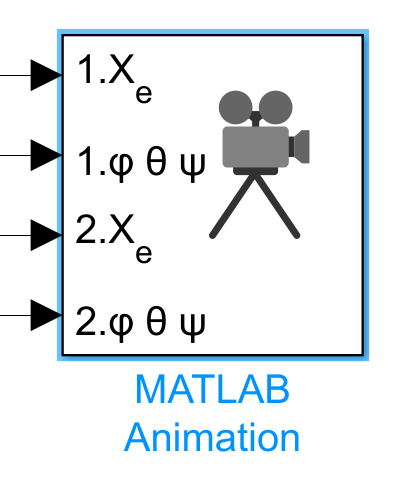
\includegraphics[width=0.35\textwidth]{./Bilder/Visual_SimBlock.png}
	\caption{Vorgefertigter 6DoF-Animations-Block in Simulink}
	\label{fig:Sim6DoFBlock}
\end{figure}

\begin{figure}[h]
	\centering
	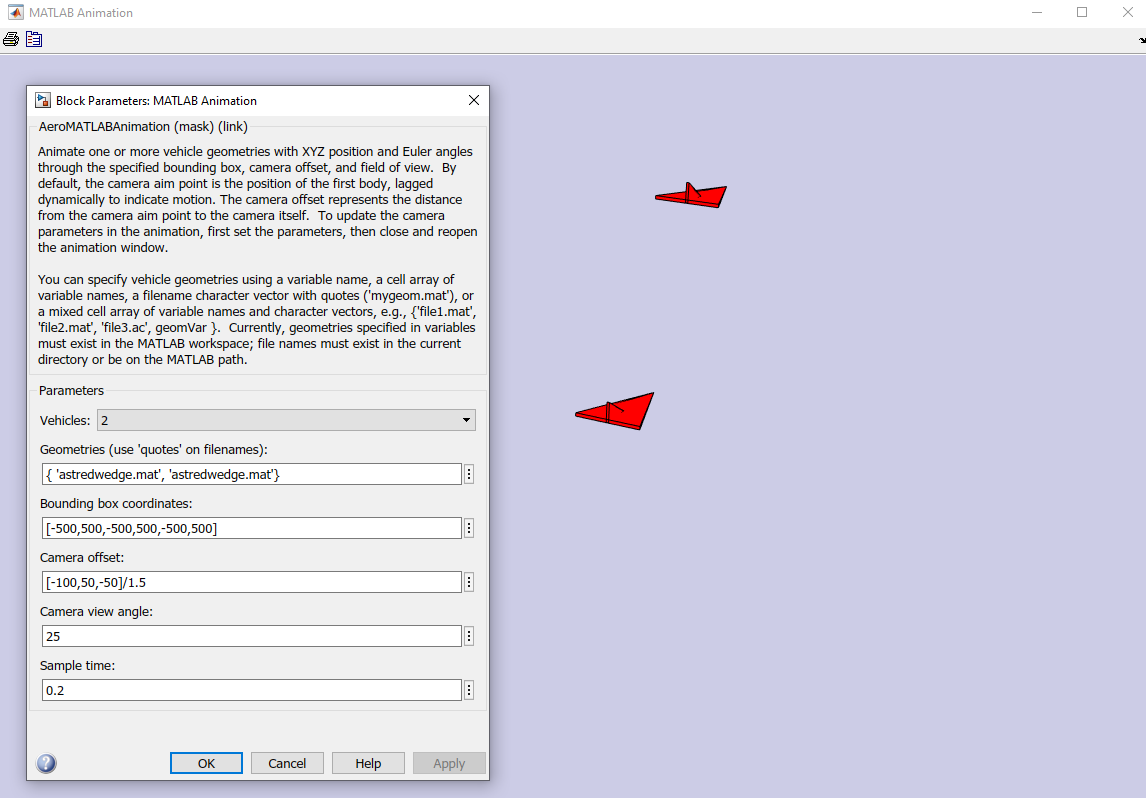
\includegraphics[width=\textwidth]{./Bilder/Visual_Sim6DoFBlockMenuBsp2.png}
	\caption{Blockparameter und Beispielanimation}
	\label{fig:Sim6DoFBlockMenuBsp}
\end{figure}
Dabei wurde für die in \ref{fig:Sim6DoFBlockMenuBsp} dargestellte Animation die voreingestellte Flugobjektgeometrie genutzt. Insgesamt betrachtet eignet sich der Animations-Block um einen Überblick über Lage, Flugbewegung und relative Position mehrerer Flugobjekte zu erhalten. Jedoch kann man die Kameraeinstellung nicht manuell während der Animation anpassen. Dies ist gerade beim Blickwinkel unpraktisch.\\
%6DoF Block:\\
%https://de.mathworks.com/help/aeroblks/6dofanimation.html\\
%Bild von Block und ergebnis\\


Eine weiter Möglichkeit der Animation bietet die Implementierung in Skriptform mit Hilfe der Aero.Animation Klasse \cite{AeroAniDoku}.
Dabei sind wieder die Flugdaten im erdfesten Koordinatensystem sowie die Eulerwinkel nötig. Zusätzlich kann über verschiedene Klassenfunktionen die Geometrie des Flugobjekts sowie die Kameraeinstellungen definiert werden. Für eine detaillierte Beschreibung der Klasse und den zugehörigen Funktionen sei auf die entsprechende Dokumentation verwiesen \cite{AeroAniDoku}.

Das in \ref{alg:MatSkripAni} dargestellte Skript beschreibt beispielhaft die Anwendung der Klasse. Der Code basiert auf dem in \cite{AeroAniOverlay} dargestellten Beispiel.
%\lstinputlisting{./inc/VisualAeroAniSkript.m}
\begin{lstlisting}[style=Matlab_colored, caption = {\Matlab-Skript zum Erstellen einer Animation über die Aero.Animation-Klasse}, label={lst:AeroAnimationSkript}]
clear;
clc;
%% Get Simulation DATA
out = sim('SixDOFSim_Vis','ReturnWorkspaceOutputs','on');
plane_1 = [out.Plane_1.time, out.Plane_1.Data];
plane_2 = [out.Plane_2.time, out.Plane_2.Data];

save('plane_1.mat', 'plane_1');
save('plane_2.mat', 'plane_2');

%% INIT Animation
% Creating instance of animation class
h = Aero.Animation; 

% Setting Framrate and Timescaling
h.FramesPerSecond = 10;
h.TimeScaling = 5;

% Creating Plane Objects
idx1 = h.createBody('pa24-250_orange.ac','Ac3d');
idx2 = h.createBody('pa24-250_blue.ac','Ac3d');

% Loading Simulation DATA
h.Bodies{1}.TimeSeriesSource = plane_1;
h.Bodies{2}.TimeSeriesSource = plane_2;

% Camera-Settings
h.Camera.PositionFcn = @doFirstOrderChaseCameraDynamics;
h.Camera.Offset = [-20,10,-10];
h.Camera.ViewAngle = 40;

% Animation
h.show();
h.play();

\end{lstlisting}

Dabei wird zunächst die Simulation gestartet um die entsprechenden Flugdaten zu erhalten. Anschließend wird eine Instanz der Animation-Klasse erzeugt. Mit Hilfe des createBody Befehls können mehrere Objekte erstellt werden. Die Geometrie wird dabei über eine entsprechende Quelldatei definiert. In dem aufgeführten Code handelt es sich bei dem Flugzeugmodel um eine Piper PA24-250 Comanche, welche von \Matlab als Beispielflugzeug genutzt wird. Ähnlich wie bei dem Animationsblock in \MatSim kann hier die Kameraeinstellungen durch relative Position und Blickwinkel bestimmt werden.

Ein Frame, der sich daraus ergebende Animation, ist in Abbildung \ref{VisualMatSk2Plane} dargestellt.
\begin{figure}[h]
	\centering
	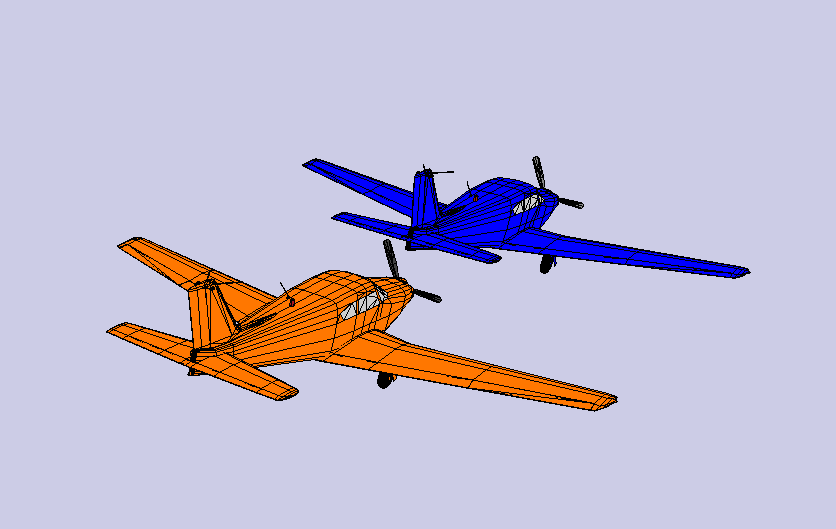
\includegraphics[width=\textwidth]{./Bilder/VisualMatSk2Plane.png}
	\caption{Beispielanimation mit Hilfe der Aero.Animaiton-Klasse}
	\label{fig:VisualMatSk2Plane}
\end{figure}
Auch hier sind die Flugbewegungen übersichtlich darstellbar aber eine handliche Anpassung des Blickwinkels ist wieder nicht gegeben.

Beide Methoden eigen sich um die relativen Bewegungen der beiden Flugzeuge zu veranschaulichen. 
Da jedoch jeweils kein Horizont oder Hintergrundobjekte implementiert sind, ist die global Flugbewegung nur schwer nachvollziehbar.


%Als Matlabskript:\\
%Ein Flugzeug:
%Skript
%Bild von zwei Flugzeugen 

%Einfache Erweiterung um weiter Flugzeuge:
%	-> Overlaying :\\
%	https://de.mathworks.com/help/aerotbx/ug/overlaying-simulated-and-actual-flight-data.html
	

%Zitate:\\
%https://de.mathworks.com/help/aerotbx/ug/aero.animation-class.html 						LABEL: AeroAniDoku\\
%https://de.mathworks.com/help/aerotbx/ug/overlaying-simulated-and-actual-flight-data.html	LABEL: AeroAniOverlay\\
%https://de.mathworks.com/help/aeroblks/6dofanimation.html									LABEL: Sim6DoFDoku\\

\section{Visualisierung mit Matlab und FlightGear}\label{app:VisualFG}
Eine weitere Möglichkeit der Darstellung bietet die in der Aero-Toolbox implementierte Schnittstelle zwischen dem Flugsimulator FlightGear und \MatSim \cite{FGBlockDoku}. Bei FlightGear handelt es sich um eine Open-Source Software welche unter anderem zu Forschungszwecken und Pilotentraining entwickelt wurde. Die Schnittstelle von \MatSim zu FlightGear bietet damit die Möglichkeit einer möglichst realistischen Visualisierung von Flugbewegungen.
In \ref{fig:VisualFGBlock} sind die dafür nötigen Simulink-Blöcke gezeigt. Der erst Block benötigt die Eulerwinkel, Längen- und Breitengrad sowie die Flughöhe. Es können aber auch wie in \ref{label} beschreiben weitere Informationen wie zum Beispiel zu Geschwindigkeiten oder Antrieb und Treibstoff hinzugefügt werden.
Diese Informationen werden dann als so genanntes net-fdm-packet ausgegeben um anschließend mit dem zweiten Block an FlightGear gesendet zu werden. Dafür definiert man in den Blockparametern ein entsprechende Port sowie eine IP Adresse (vgl. \ref{fig:VisualFGBlockParam}).
Es gibt auch einen vorkonfigurierten Block, welcher die beiden beschriebenen Blöcke enthält. Da dieser jedoch zusätzlich einen Set-Pace-Block beinhaltet kann er nicht mehrfach in einem \MatSim Modell genutzt werden. Somit ist er nicht für Anwendungen geeignet bei denen mehrere Flugzeuge dargestellt werden sollen.
\begin{figure}[h]
	\centering
	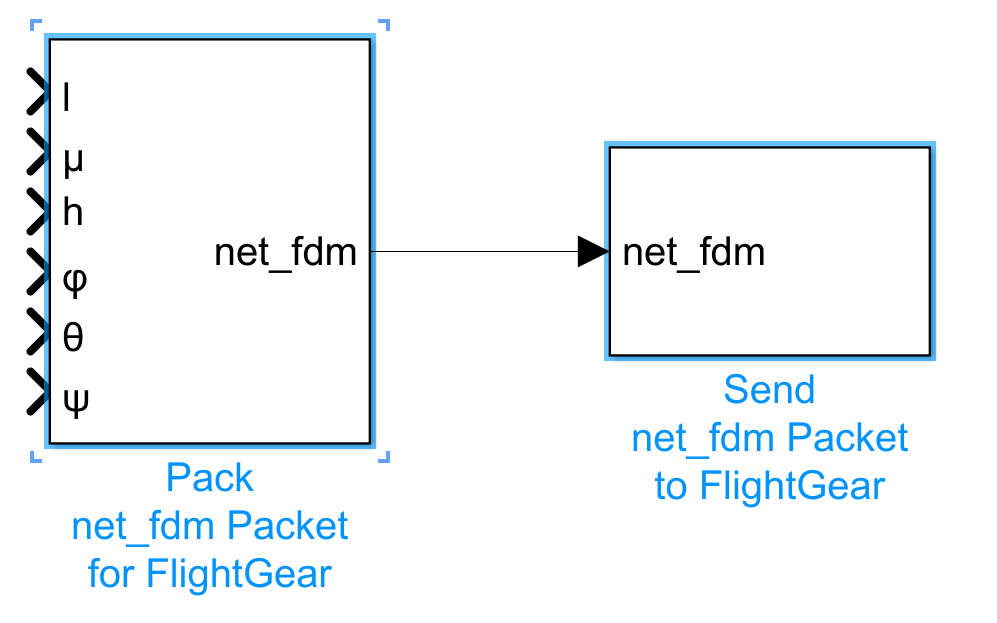
\includegraphics[width=\textwidth]{./Bilder/Visual_FGBlock.png}
	\caption{Simulink-Blöcke für Schnittstelle zu Flugsimulator FlightGear}
	\label{fig:VisualFGBlock}
\end{figure}
\begin{figure}[h]
	\centering
	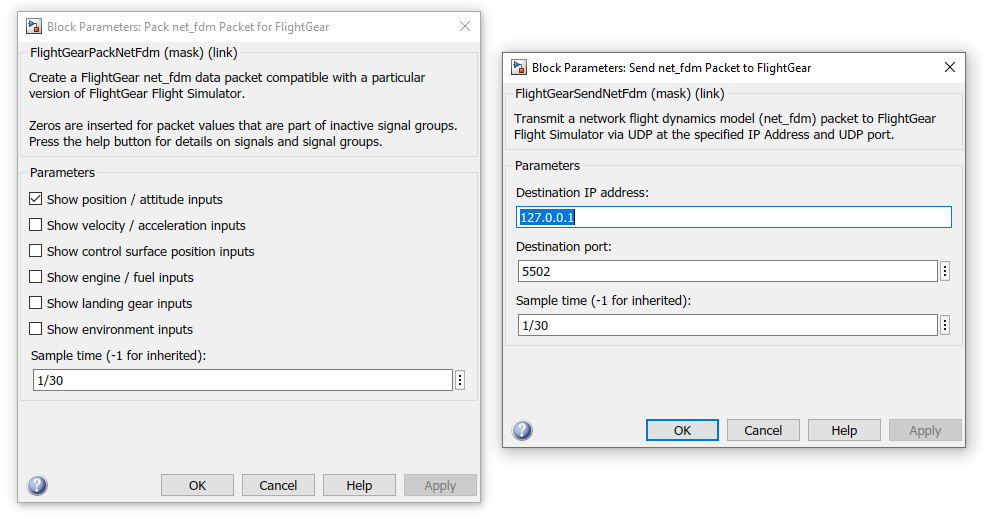
\includegraphics[width=\textwidth]{./Bilder/Visual_NetFdmBlockParam.png}
	\caption{Blockparameter für Simulink/FlightGear-Schnittstelle}
	\label{fig:VisualFGBlockParam}
\end{figure}

In FlightGear müssen dann die äquivalenten Einstellungen getroffen werden. Hierfür gibt es eine Kommandozeile in welche die Befehle in Codeform formuliert werden können. 
Möchte man mehrere Flugzeuge simulieren so kann man den Multiplayer-Modus nutzen um mehrere FlightGear-Instanzen zu verknüpfen. Dies geschieht entweder lokal oder auf einem offiziellen Server von FlightGear. Eine detailliertere Ausführung zu den möglichen Multiplayer-Einstellungen ist in \cite{How2Multi} zu finden.
Nachfolgender Code beschreibt beispielhaft die nötigen Eingaben in die FlightGear-Komandozeile.\\

Plane 1: --fdm=null --native-fdm=socket,in,30,localhost,5502,udp --multiplay=out,10,127.0.0.1,5000 --multiplay=in,10,127.0.0.1,5001 --callsign=Test1 \\

Plane 2: --fdm=null --native-fdm=socket,in,30,localhost,5503,udp --multiplay=out,10,127.0.0.1,5001 --multiplay=in,10,127.0.0.1,5000 --callsign=Test2\\


Plane 1: --fdm=null --native-fdm=socket,in,30,localhost,5502,udp --native-ctrls=socket,out,30,localhost,5505,udp --multiplay=out,10,mpserver01.flightgear.org,5000 --multiplay=in,30,,5000 --callsign=Test1 \\

Plane 2: --fdm=null --native-fdm=socket,in,30,localhost,5503,udp --native-ctrls=socket,out,30,localhost,5505,udp --multiplay=out,10,mpserver01.flightgear.org,5000 --multiplay=in,30,,5001 --callsign=Test2 \\

In Abbildung \ref{fig:VisualFG2Planes} ist ein Frame aus der FlightGear Animation gezeigt, welcher mit dieser Methode konzipiert wurde.
\begin{figure}[h]
	\centering
	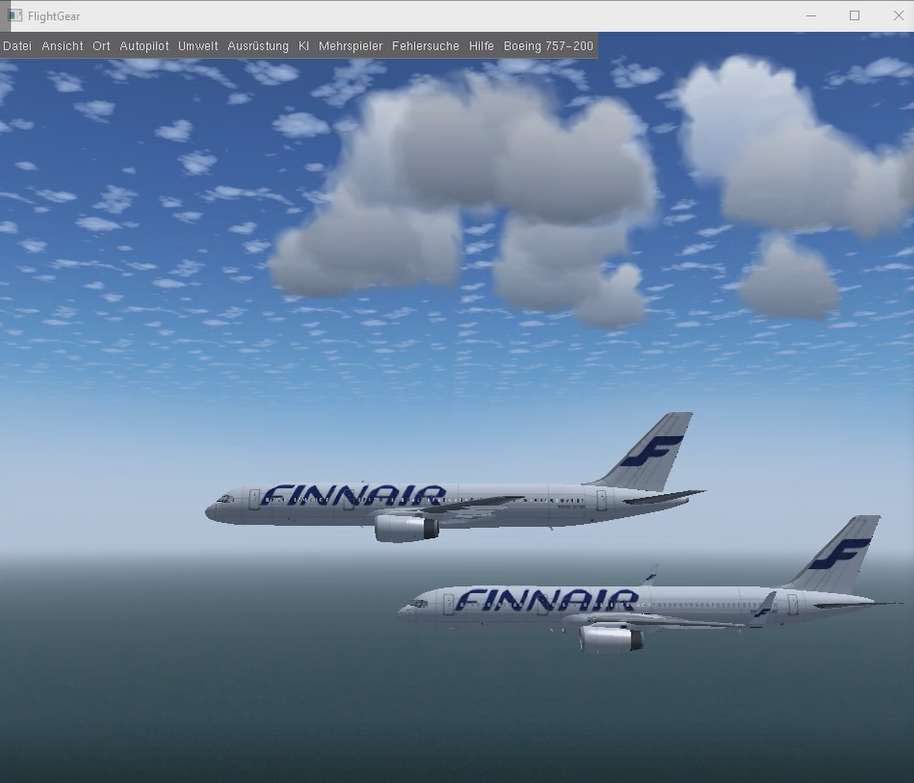
\includegraphics[width=\textwidth]{./Bilder/Visual_FG2Planes.png}
	\caption{Beispielanimation mit FlightGear}
	\label{fig:VisualFG2Planes}
\end{figure}
Aus einer breiten Bibliothek an Flugzeugen kann das für die Simulation benötigte ausgewählt werden. Zudem ist des möglich den Blickwinkel während der Animation anzupassen. Des weiteren ist durch den Horizont und die Wolken die Flugbahn der Flugzeuge besser nachvollziehbar. 

Jedoch tritt ein gravierendes Problem auf. Die Darstellung ruckelt und ist zeitlich verschoben. Damit ist sie für diese Arbeit ungenügend. Denn die Performance der Regelung kann nicht veranschaulicht werden, wenn die Flugzeuge in der Animation mehrere Meter hin und her springen. Die Ursache hierfür ist eine Asynchronität von \MatSim und den verschiedenen FlightGear-Instanzen.
Im Rahmen dieser Arbeit konnte dieses Problem nicht gelöst werden. In \cite{FGForum} wird ein mögliche Methode beschreiben um das Problem zu umgehen.
Dabei wird eine für diesen Zweck angepasste Version von FlightGear genutzt um die gesendeten Pakete auszulesen und mit einem Zeitstempel zu versehen. Somit kann eine flüssigere Animation erzielt werden.


%-> FG Blöcke + Impl Bsp:\\
%https://nl.mathworks.com/help/aeroblks/working-with-the-flight-simulator-interface.html
%
%Auch möglihc mehrer Flugzeuge dafür MultiPlayer\\
%Sub von FG Block da set Pace\\
%
%
%=> Problem keine saubere darstellung: Lag plus jitter\\
% Ursache: asynchronität von Packagerate Sim vs FG \\
% versuchte Lösungsansätze:\\
%  -rechenpower\\
%  -aufnahmen\\
%  -nicht lokal sondern Offi server\\
%  -Lag und Synch einstellungen\\
%  -red. der output rate / frame rate\\
%  
%  Nichts desto Trotz konnte im rahmen dieser Arbeit keine Lösung erarbeitet werden.\\
%
%
%Bilder:\\
%-Block in Matlab \\
%	.einfach\\
%    .für 2 Flugzeuge -> Set Pace Block\\
%- Einstellungsmenü in FG\\
%- flug in FG\\

 	
%REF:\\
%-Forum Markus: https://forum.flightgear.org/viewtopic.php?f=27&t=38421 	LABEL: FGForum\\
%-HowToMulti: https://wiki.flightgear.org/Howto:Multiplayer					LABEL: How2Multi\\

